\documentclass{article}%
\usepackage[T1]{fontenc}%
\usepackage[utf8]{inputenc}%
\usepackage{lmodern}%
\usepackage{textcomp}%
\usepackage{lastpage}%
\usepackage{geometry}%
\geometry{left=3cm,right=3cm,bottom=2cm,top=1cm}%
\usepackage[russian]{babel}%
\usepackage{amsmath}%
\usepackage{amssymb}%
\usepackage{amsfonts}%
\usepackage{mathtext}%
\usepackage{graphicx}%
%
%
%
\begin{document}%
\normalsize%
\begin{center}%
.\\%
\vspace{12cm}%
\textbf{Лабораторная работа № 3.03: Определение удельного заряда электрона}%
\end{center}%
\begin{center}%
Исхаков Камиль Фархатович%
\end{center}%
\begin{center}%
\today%
\end{center}%
\newpage%
\section{Основные формулы:}%
\label{sec:}%

%
Магнитная индукцию внутри соленоида:\begin{displaymath} B_c = \mu_0 I_c N \frac{1}{\sqrt{(l^2+d^2)}}\end{displaymath}%
\newline%
где $\mu_0 =  4 \pi 10^{-7} $ Гн/м – магнитная постоянная, $N$ – число витков соленоида, $l$ – его длина, $d$ – его диаметр.%
\newline%
Формула удельного заряда:\begin{displaymath}\frac{e}{m} = \frac{8 U}{B_c^2 r_a^2}\end{displaymath}%
\newline%
где $e$ – заряд электрона, $m$ – его масса, $r_a$ – радиус анода, $U$ – анодное напряжение%
\newline%
\section{Расчеты:}%
\label{sec:}%

%


\begin{figure}[h!]%
\centering%
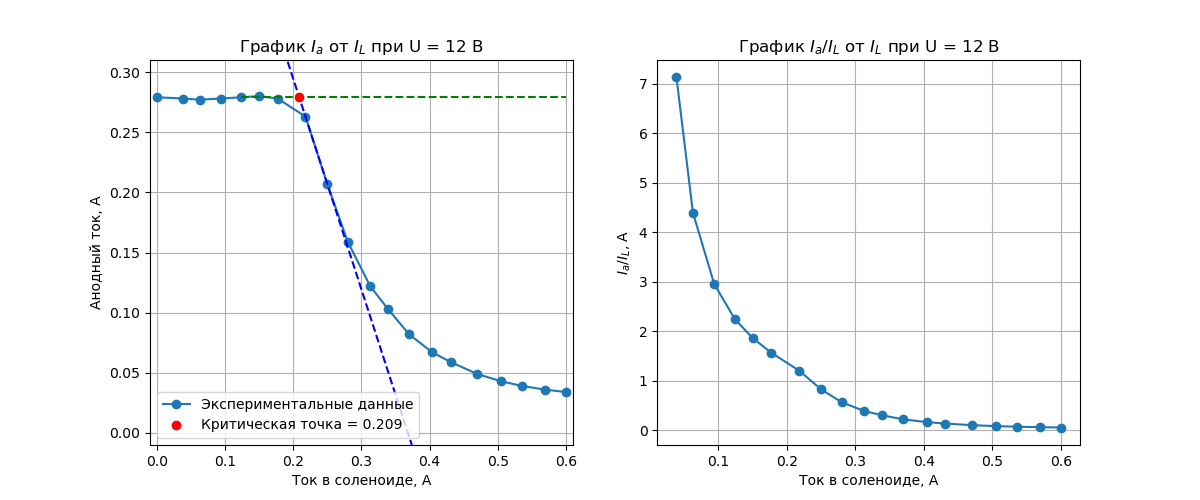
\includegraphics[width=400px]{combined_plot_U_12.png}%
\caption{Комбинированный график зависимости анодного тока и $I_a/I_L$ от тока в соленоиде при $U$ = 12 В}%
\end{figure}

%


\begin{figure}[h!]%
\centering%
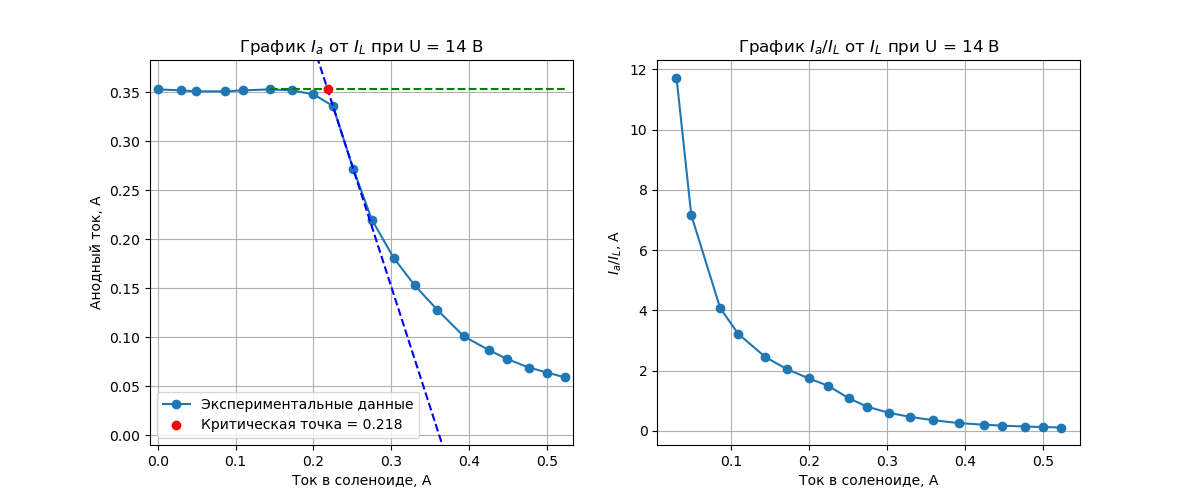
\includegraphics[width=400px]{combined_plot_U_14.png}%
\caption{Комбинированный график зависимости анодного тока и $I_a/I_L$ от тока в соленоиде при $U$ = 14 В}%
\end{figure}

%


\begin{figure}[h!]%
\centering%
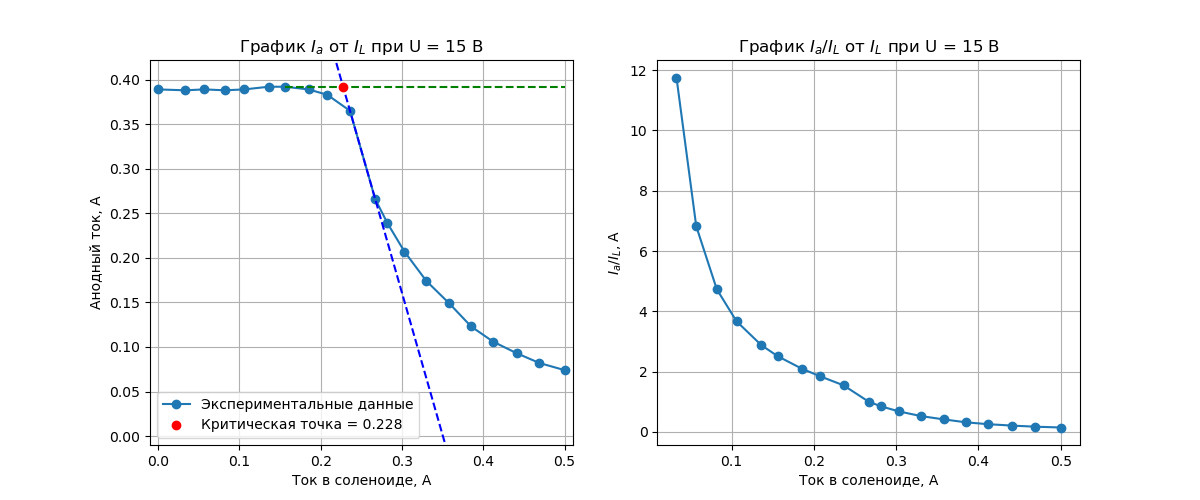
\includegraphics[width=400px]{combined_plot_U_15.png}%
\caption{Комбинированный график зависимости анодного тока и $I_a/I_L$ от тока в соленоиде при $U$ = 15 В}%
\end{figure}

%
Получившиеся графики в полной мере наглядно показывают когда траектория электронов становится касательной к поверхности анода.%
\section{Результаты эксперимента}%
\label{sec:}%
\begin{tabular}{|c|c|c|c|}%
\hline%
$U$, В&$I_{L_c}$, мА&$B_c$, мТл&$e/m$, Кл/кг\\%
\hline%
12&0.209&7.96&$1.683 \cdot 10^{11}$\\%
\hline%
14&0.218&8.216&$1.844 \cdot 10^{11}$\\%
\hline%
15&0.228&8.617&$1.796 \cdot 10^{11}$\\%
\hline%
\end{tabular}

%
 \vspace{0.5cm} Среднее значение $\langle \frac{e}{m} \rangle$: \text{ $1.774 \cdot 10^{11}$ Кл/кг}%


\begin{figure}[h!]%
\centering%
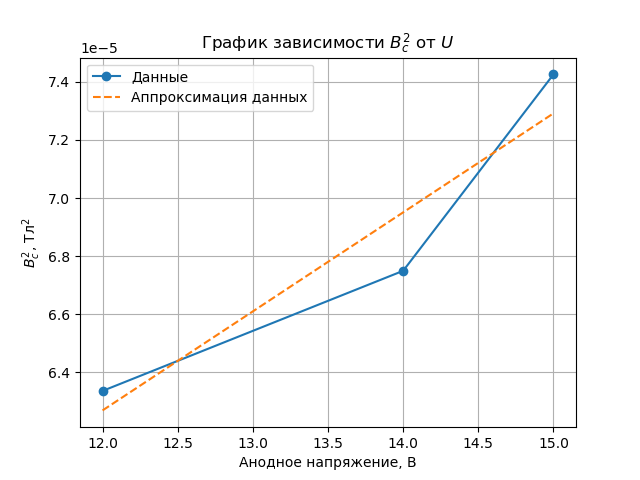
\includegraphics[width=400px]{Bc2_vs_U.png}%
\caption{График зависимости $B_c^2$ от анодного напряжения $U$}%
\end{figure}

%
 Угловой коэффициент аппроксимирующей прямой $k$ = $0.341 \cdot 10^{-5}$.%
 \\ \vspace{1cm} Следовательно, $\frac{e}{m}$ = $\frac{8 k}{r_a^2}$ =  $2.608 \cdot 10^{11}$ Кл/кг.%
\section{Оценка погрешностей}%
\label{sec:}%
Оценим погрешность удельного заряда электрона: %
 Вычислим для каждого из значений анодного напряжения и критического тока:%
$$\Delta \left( \frac{e}{m} \right) = \sqrt{ \left( \frac{\partial \left( \frac{e}{m} \right)}{\partial U} \Delta U \right)^2 + \left( \frac{\partial \left( \frac{e}{m} \right)}{\partial B_c} \Delta B_c \right)^2 + \left( \frac{\partial \left( \frac{e}{m} \right)}{\partial r_a} \Delta r_a \right)^2 }$$%
$$\frac{\partial \left( \frac{e}{m} \right)}{\partial U} = \frac{8}{B_c^2 r_a^2}$$%
$$\frac{\partial \left( \frac{e}{m} \right)}{\partial B_c} = -\frac{16U}{B_c^3 r_a^2}$$%
$$\frac{\partial \left( \frac{e}{m} \right)}{\partial r_a} = -\frac{16U}{B_c^2 r_a^3}$$%
Оценим погрешность для U = 12 В: %
$$\Delta \left( \frac{e}{m} \right) = \sqrt{ \left( \frac{8 \Delta U}{B_c^2 r_a^2} \right)^2 + \left( \frac{16U \Delta B_c}{B_c^3 r_a^2} \right)^2 + \left( \frac{16U \Delta r_a}{B_c^2 r_a^3} \right)^2 } = \text{$1.131 \cdot 10^{10}$} \text{Кл/кг}$$%
Относительная погрешность: 6.37\%%
\newline%
Оценим погрешность для U = 14 В: %
$$\Delta \left( \frac{e}{m} \right) = \sqrt{ \left( \frac{8 \Delta U}{B_c^2 r_a^2} \right)^2 + \left( \frac{16U \Delta B_c}{B_c^3 r_a^2} \right)^2 + \left( \frac{16U \Delta r_a}{B_c^2 r_a^3} \right)^2 } = \text{$1.236 \cdot 10^{10}$} \text{Кл/кг}$$%
Относительная погрешность: 6.97\%%
\newline%
Оценим погрешность для U = 15 В: %
$$\Delta \left( \frac{e}{m} \right) = \sqrt{ \left( \frac{8 \Delta U}{B_c^2 r_a^2} \right)^2 + \left( \frac{16U \Delta B_c}{B_c^3 r_a^2} \right)^2 + \left( \frac{16U \Delta r_a}{B_c^2 r_a^3} \right)^2 } = \text{$1.203 \cdot 10^{10}$} \text{Кл/кг}$$%
Относительная погрешность: 6.78\%%
\newline

%
Получившиеся относительные погрешности для каждого из конкретного значения напряжения оказались приблизительно равны 6 процентам, что является допустимым.%
\section{Выводы}%
\label{sec:}%

%
Табличное значение удельного заряда электрона:\begin{displaymath}\frac{e}{m} = 1,76\cdot10^{11} \textit{ Кл/кг}\end{displaymath}%
\newline%
В ходе работы был определен удельный заряд электрона. Табличное и экспериментальное значение удельного заряда электрона в нашем случае получилось почти идентичными. Во время выполнения всей лабораторной работы значения получались вполне реалистичными, кроме задания с построением зависимости $B^2_c$ от $U$, поскольку значение удельного заряда, вычисленный через коэффициент наклона прямой оказалось в полтора раза больше табличного значения. Расхождение теоретического значения удельного заряда от экспериментального может быть из-за влияния облака заряда, накапливающегося в диоде. %
\newline%
\end{document}